\section{"2" Определение физико-механических свойств поверхности}

\begin{frame}[t]{Определение физико-механических свойств}
    \framesubtitle{}
    \small
    Определить процентное соотношение твердых, упругих и пластичных свойств пройденной поверхности

    \textbf{Метод решения}: машинное обучение, Метод Опорных Векторов (SVM)

    \textbf{Алгоритм}: Создается \underline{установка} для обучения. \underline{Обучение}: робот ходит по различным типам поверхностей фиксированное количество касаний поверхности с постоянной угловой скоростью. Модель обучается на 80\% данных с помощью ядра PUK7. \underline{Тестирование}: происходит на оставшихся 20\%.  Используются \textbf{метрики} меткости, точности, полноты и F1-счета.

    \begin{columns}[T,onlytextwidth]
        \begin{column}{0.44\textwidth}
            \textbf{Входные данные}: данные с внутренних датчиков робота

            \textbf{Выходные данные}: процентное соотношение упругих, твердых и пластичных свойств пройденной поверхности

            \textbf{Допустимая ошибка}: 20\% - точность

            \textbf{Предположения}: 1) На рисунке.

        \end{column}
        \begin{column}{0.54\textwidth}
            \vspace{-0.5cm}
            \begin{figure}[H]
                \begin{subfigure}[b]{0.3\textwidth}
                    \centering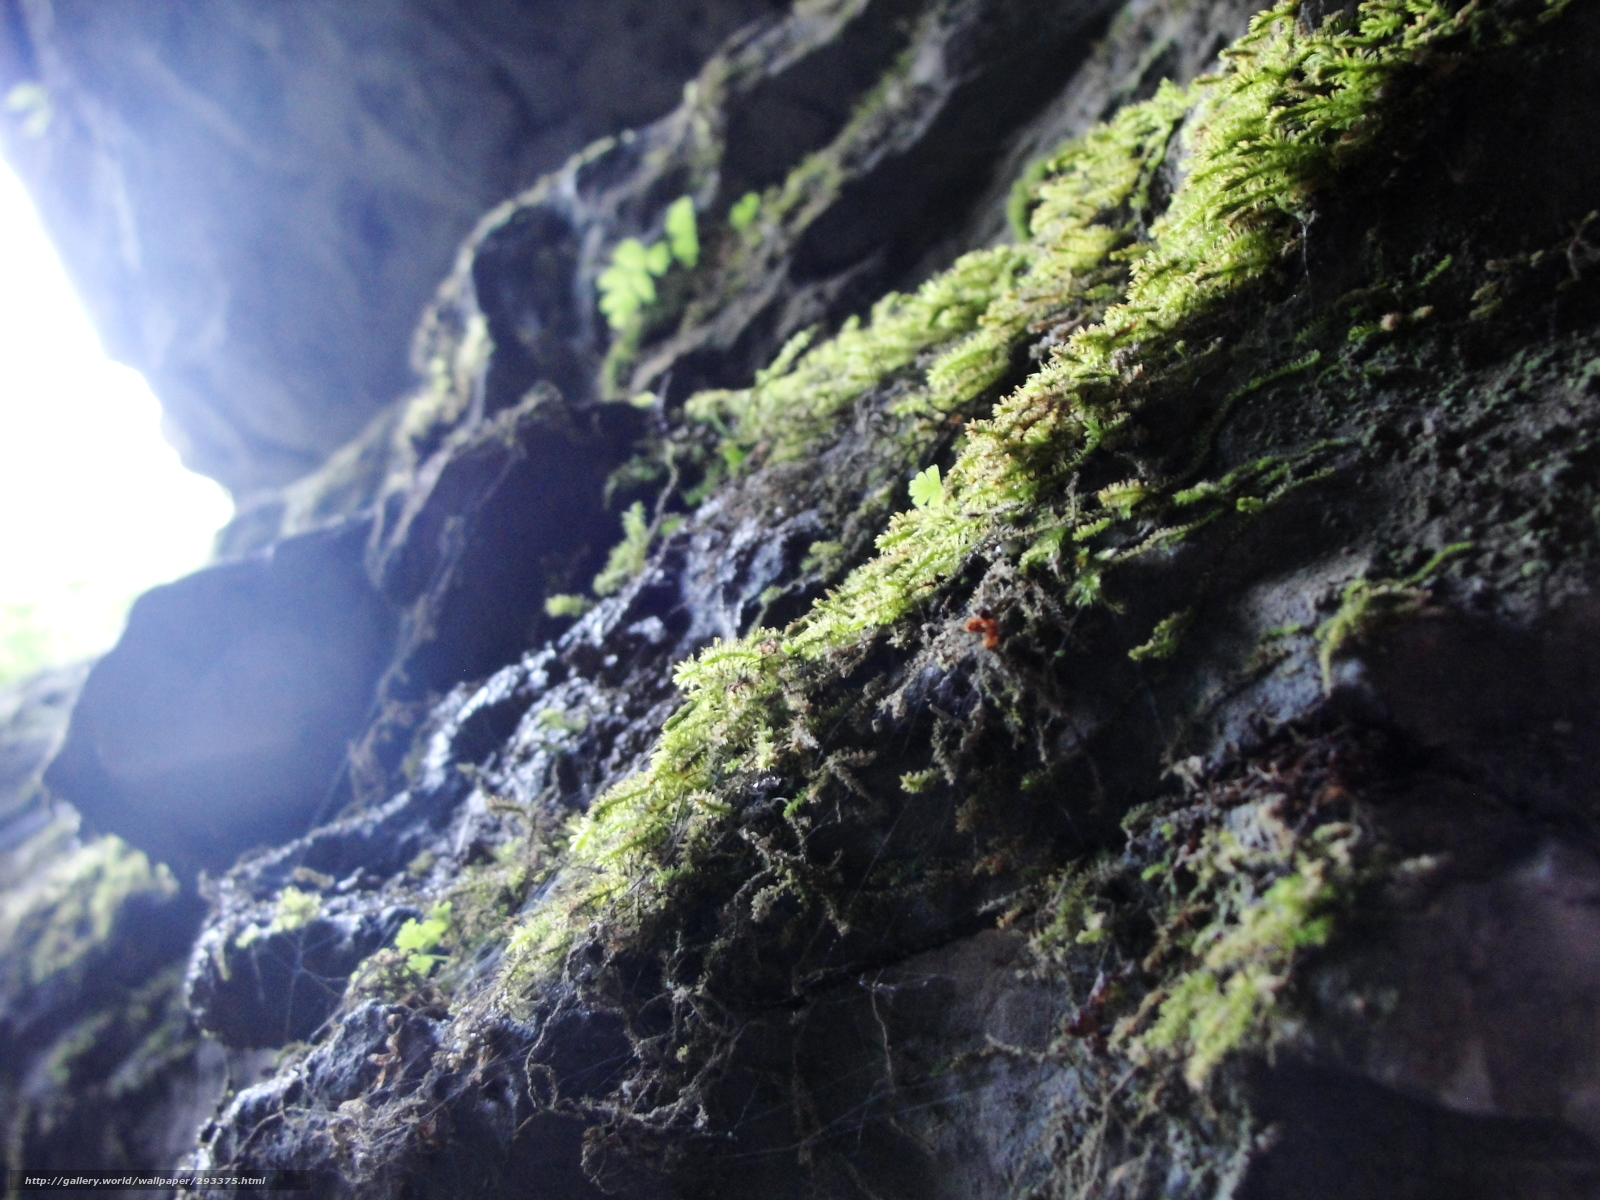
\includegraphics[height=1.5cm,width=1\textwidth,keepaspectratio]{surface_types/moss.jpg}
                \end{subfigure}
                \hfill
                \begin{subfigure}[b]{0.3\textwidth}
                    \centering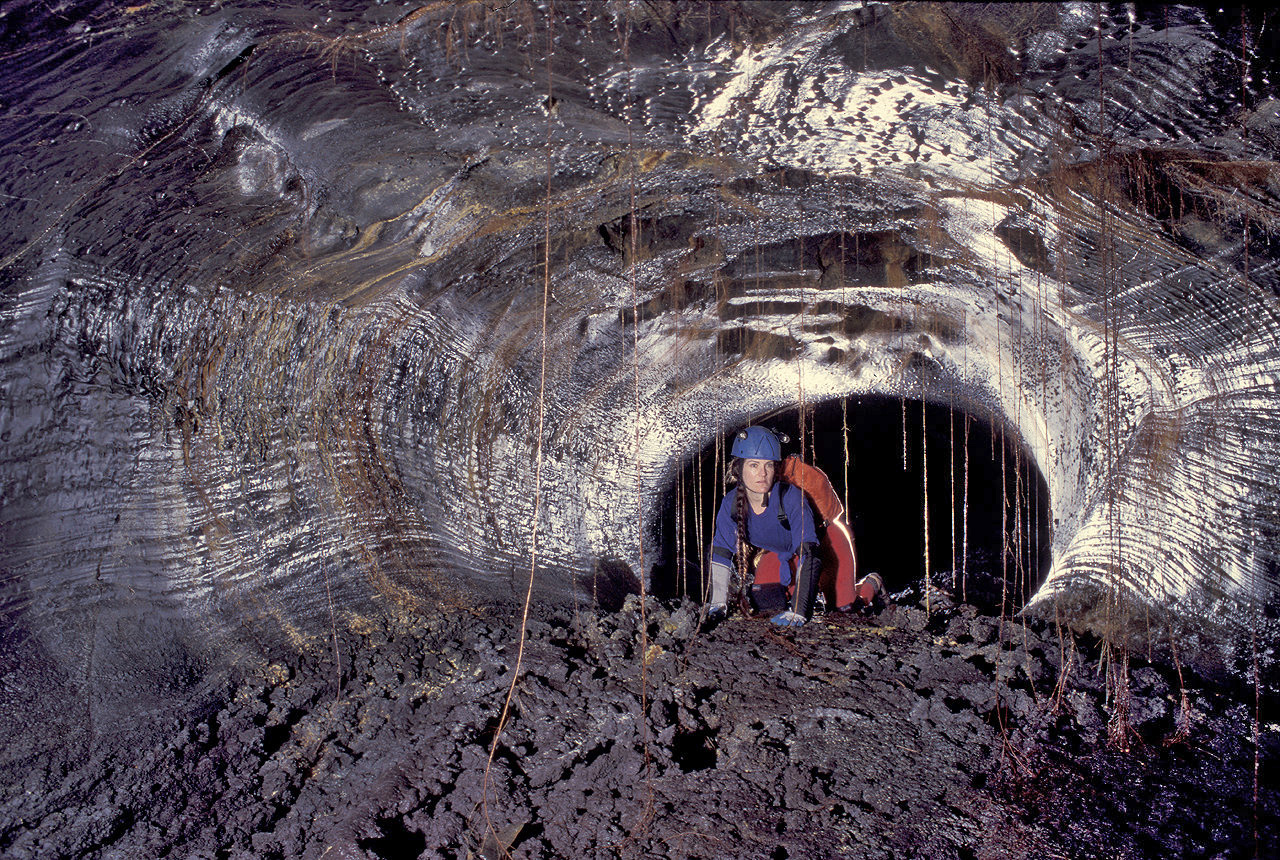
\includegraphics[height=1.5cm,width=1\textwidth,keepaspectratio]{surface_types/lava.jpg}
                \end{subfigure}
                \hfill
                \begin{subfigure}[b]{0.3\textwidth}
                    \centering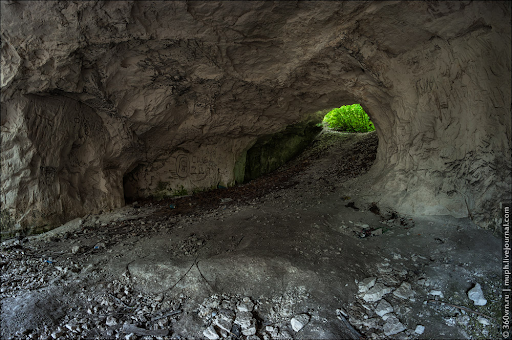
\includegraphics[height=1.5cm,width=1\textwidth,keepaspectratio]{surface_types/moul.png}
                \end{subfigure}

                \begin{subfigure}[b]{0.3\textwidth}
                    \centering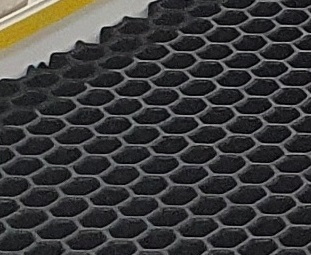
\includegraphics[height=1.5cm,width=1\textwidth,keepaspectratio]{surface_types/rubber.JPG}
                \end{subfigure}
                \hfill
                \begin{subfigure}[b]{0.3\textwidth}
                    \centering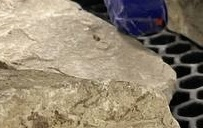
\includegraphics[height=1.5cm,width=1\textwidth,keepaspectratio]{surface_types/rock.jpg}
                \end{subfigure}
                \hfill
                \begin{subfigure}[b]{0.3\textwidth}
                    \centering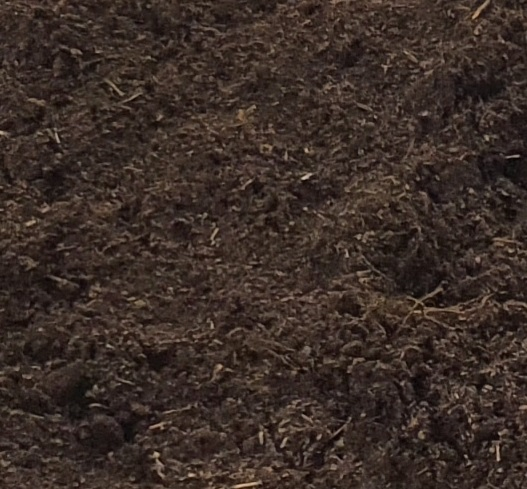
\includegraphics[height=1.5cm,width=1\textwidth,keepaspectratio]{surface_types/zemlya.jpg}\\
                \end{subfigure}
                \vspace{-0.3cm}
                \caption{Эталоны упругой, твердой и пластичной поверхностей}
            \end{figure}
        \end{column}
    \end{columns}
\end{frame}

\note{\small \setlength{\parindent}{20pt}

Решив задачи 3 и 4, то есть имея разработанный сенсор и узел с ногой робота, возможно решать задачу определения физико-механических свойств поверхности. Для получения более точных результатов, было решено решать данную задачу натурно.

Любой материал можно описать с помощью вязко-упруго-пластичной модели, но их сложно померить и еще сложнее интерпретировать. Поэтому более целесообразно классифицировать объекты, которые использовались как эталонно упругие, твердые и пластичные *тык*. Аналогом мха --- эталона упругих свойств является резина, твердой --- камень, а пластичной --- земля. Результатом работы алгоритма получается процентное соотношение  упругих, твердых и пластичных свойств.

Для решения задачи классификации используется метод опорных векторов (SVM). Данные собирались так. Робот ходит по различным типам поверхностей фиксированное количество касаний поверхности с постоянной угловой скоростью. Данные с внутренних датчиков, о которых будет разговор далее, собираются. Потом происходит обучение и тестирование. Использовались классические критерии для данного типа задачи: меткость, точность, полнота и F1-счет. Это классические метрики оценки точности обученной модели.
}

\begin{frame}[t]{Стенд}
    \framesubtitle{}
    \begin{figure}[H]
        \begin{subfigure}[t]{0.33\textwidth}
            \centering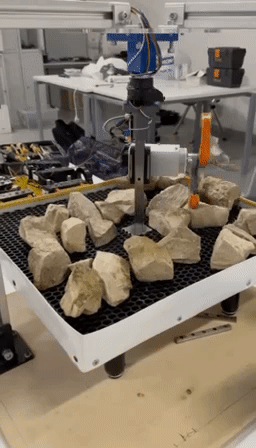
\includegraphics[height=5cm,width=1\textwidth,keepaspectratio]{s_shape_leg/rockk.png}
            \caption*{Установка}
        \end{subfigure}
        \begin{subfigure}[t]{0.33\textwidth}
            \centering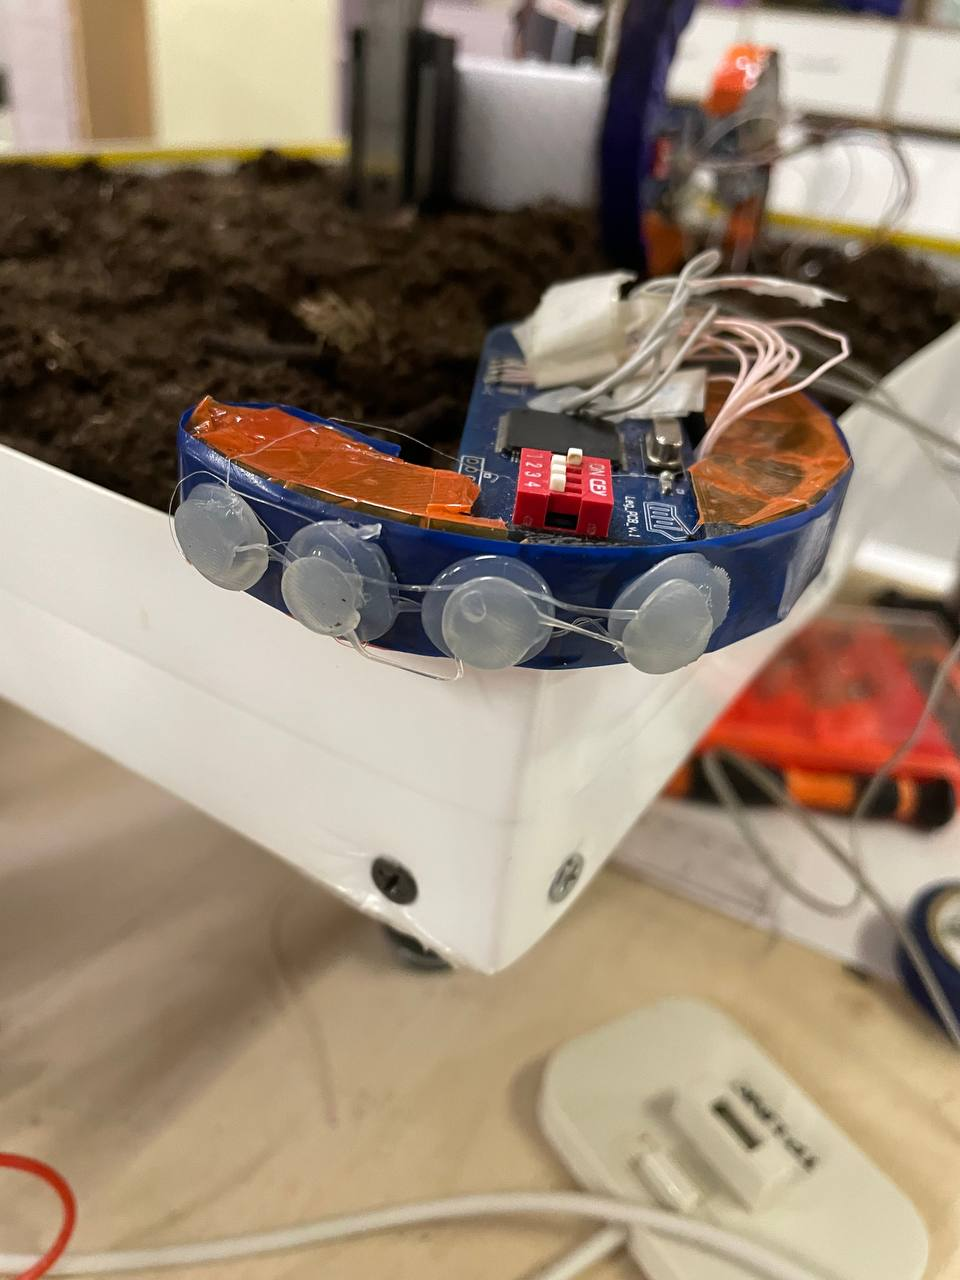
\includegraphics[height=5cm,width=1\textwidth,keepaspectratio]{s_shape_leg/socks.jpg}
            \caption*{Нога робота с установленными сенсорами}
        \end{subfigure}
        \begin{subfigure}[t]{0.33\textwidth}
            \centering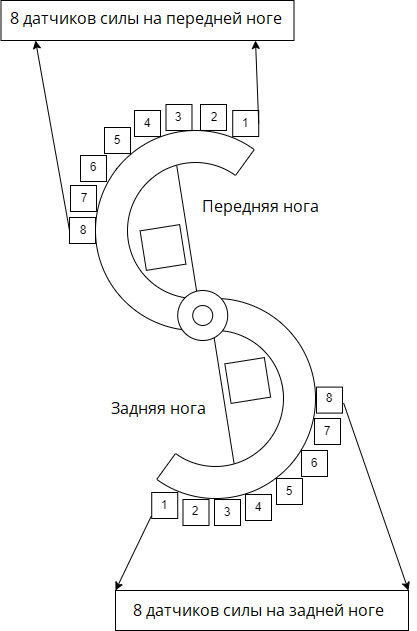
\includegraphics[height=5cm,width=1\textwidth,keepaspectratio]{s_shape_leg/leg_design.png}
            \caption*{Схематическое распределение сенсоров на ноге}
        \end{subfigure}
    \end{figure}
\end{frame}

\note{\small \setlength{\parindent}{20pt}

На экране представлен стенд *тык*, нога робота, на которую установлены датчики силы *тык*, а также способ установки сенсоров на ногу *тык*. 

Нужно отметить, что во время испытаний, пришел к выводу, что максимум нужно 5 сенсоров, а не 8, как указано на рисунке справа.

На видео показана работа стенда во время обучения.
}

\begin{frame}[t]{Метод опорных векторов}
    \framesubtitle{}
    \small

    \begin{columns}[T,onlytextwidth]
        \begin{column}{0.49\textwidth}
            \vspace{-0.5cm}
            \begin{align}
                f(x) = w^T x + b
            \end{align}

            \vspace{-0.2cm}

            где $w$ --- весовой вектор, $b$ --- смещение,

            $x$ --- \textbf{входной вектор}:

            (1) Частота движения ног\\
            (2-12) Данные с датчика силы\\
            (13-16) Данные крутящего момента двигателя\\
        \end{column}
        \begin{column}{0.49\textwidth}
            Ядро на основе функции Пирсона VII:
            \begin{align}
                K(x, y) = (1 + ((||x - y||^2)/\sigma^2)^\omega)^{(-1/\omega)}
            \end{align}

            \vspace{-0.2cm}

            Где $x$, $y$ --- векторы во входном пространстве, $||x - y|||$ --- евклидово расстояние между $x$ и $y$, $\sigma$ --- масштабный параметр; $\omega$ --- это параметр формы.
        \end{column}
    \end{columns}
    \vspace{-0.4cm}
    \begin{figure}[H]
        \begin{subfigure}[t]{0.49\textwidth}
            \centering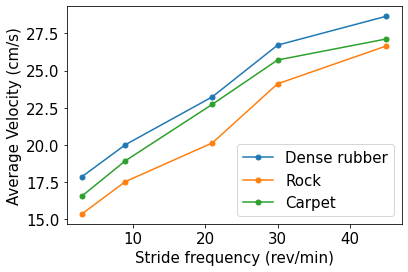
\includegraphics[height=3cm,width=1\textwidth,keepaspectratio]{../images/s_shape_leg/avg_lin_vel_rev_min.png}
            \caption*{Зависимость угловой скорости от линейного перемещения}
        \end{subfigure}
        \begin{subfigure}[t]{0.49\textwidth}
            \centering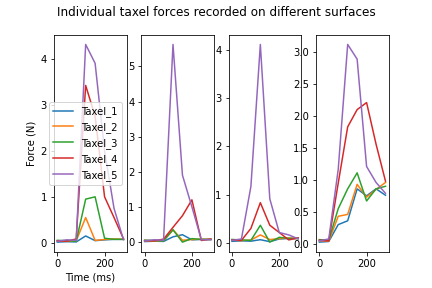
\includegraphics[height=3cm,width=1\textwidth,keepaspectratio]{../images/s_shape_leg/TaxelIndForce.png}
            \caption*{Распределение силы нажатия на каждый сенсор}
        \end{subfigure}
    \end{figure}
\end{frame}

\note{\small \setlength{\parindent}{20pt}

Метод опорных векторов --- алгоритм обучения с учителем. описывается следующей формулой *тык*. Главная цель SVM как классификатора --- найти уравнение разделяющей гиперплоскости. 

Входной вектор включал в себя частоту движения ног *тык*, так как показано на рисунке справа - он может критерием определения, так как при одинаковой частоте вращения, линейное перемещение разное. 

Информация с датчиков силы *тык*. На графиках одно нажатие ноги на резину, камень и землю. На оси х --- время, на оси ординат --- сила на каждом конкретном датчике силы. Как видно, разный характер распределения сил в зависимости от материала. также с мотора - основные показания.

Также снимались данные о моменте с мотора.

Так как у нас задача нелинейная, то использовался kernel trick. Функция ядра обычно преобразует обучающий набор данных таким образом, что нелинейная поверхность принятия решений способна преобразовываться в линейное уравнение в пространствах большего числа измерений. Для этого использовалась функция Пирсона VII.
}

\begin{frame}[t]{Результаты}
    \framesubtitle{}
    \begin{columns}[T,onlytextwidth]
        \begin{column}{0.49\textwidth}
            \begin{table}[H]
                \resizebox{\linewidth}{!}{%
                    \begin{tabular}{|c|c|c|c|c|}
                        \cline{3-5}
                        \multicolumn{1}{l}{}                     & \multicolumn{1}{l|}{} & \multicolumn{3}{c|}{\textbf{Предсказанный класс}}                                                                                           \\
                        \cline{3-5}
                        \multicolumn{1}{l}{}                     &                       & Камень                                            & Резина                                     & Земля                                      \\
                        \hline
                        \multirow{3}{*}{{\textbf{Истин. класс}}} & Камень                & {\cellcolor[rgb]{0.741,0.843,0.929}}84.0\%        & 2.56\%                                     & 13.44\%                                    \\
                        \hhline{|~----|}
                                                                 & Резина                & 20.1\%                                            & {\cellcolor[rgb]{0.741,0.843,0.929}}67.8\% & 12.1\%                                     \\
                        \hhline{|~----|}
                                                                 & Земля                 & 1.0\%                                             & 18.9\%                                     & {\cellcolor[rgb]{0.741,0.843,0.929}}80.1\% \\
                        \hline
                    \end{tabular}
                }
                \caption{Результаты обученного классификатора опорных поверхностей}
            \end{table}

            Камень --- эталон твердых свойств поверхности;\\
            Резина --- эталон упругих свойств;\\
            Земля --- эталон пластичных свойств.
        \end{column}
        \begin{column}{0.49\textwidth}
            \begin{figure}[H]
                \centering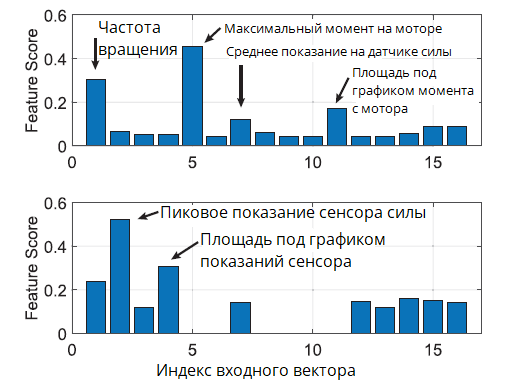
\includegraphics[height=5cm,width=1\textwidth,keepaspectratio]{../images/s_shape_leg/feature_score.png}
                \caption*{Гистограмма влияния входных данных на результат предсказания}
            \end{figure}
        \end{column}
    \end{columns}
\end{frame}

\note{\small \setlength{\parindent}{20pt}

На слайде представлены результаты классификации опорных поверхностей *тык*. 

Ее можно интерпретировать следующим образом. В камне 84 процента твердых свойств, 2.5 упругих и 13.44 пластичных. В резине --- 20 процентов твердых, 67.8 упругих и 12.1 --- пластичных.

Не менее важный вопрос, какие данные оказали самый весомый вклад в определении физико-механических свойств. Для этого была построенная гистограмма влияния входных данных *тык*.

Верхний график --- когда брались все данные, нижний --- без показаний с мотора.

На основе гистограммы можно увидеть, что момент на моторе и частота вращения имеют большее влияние на предсказание, чем данные о силе нажатия.
}